%\documentclass{beamer}

\documentclass[10pt]{beamer} 
\usetheme[pageofpages=of,% String used between the current page and the
          % total page count.
          alternativetitlepage=true,% Use the fancy title page.
          %titlepagelogo=coca,% Logo for the first page.
          titleline=true
          ]{Torino}
%\usetheme{Frankfurt}
\usecolortheme{chameleon}

\usepackage{graphicx,hyperref,url}
\usepackage[utf8]{inputenc}
\usepackage[T1]{fontenc}
\usepackage[portuges,brazilian]{babel}
%%%\usepackage{wrapfig}
\usepackage{caption}
\usepackage{subfigure}
%\usepackage{subcaption}
\usepackage{latexsym}
\usepackage{amssymb, amsmath}
\usepackage{multicol}
\usepackage{pifont}%,bbding}%%,dingbat} %%% ver manual de simbolos
\usepackage[final]{listings}
\usepackage{comment}


\definecolor{azulclaro}{rgb}{0.9,0.9,0.9}
\definecolor{mygreen}{rgb}{0,0.6,0}
\definecolor{mygray}{rgb}{0.5,0.5,0.5}
\definecolor{mymauve}{rgb}{0.58,0,0.82}
\definecolor{darkgray}{rgb}{.4,.4,.4}
\definecolor{purple}{rgb}{0.65, 0.12, 0.82}

\newcommand{\minizinc}{MiniZinc}

\lstset{ 
  %  label={pgm_ex01},
    backgroundcolor=\color{azulclaro}, 
    language=Erlang, %%Miranda,%%Perl,%%%Python, %%Mercury,
    showstringspaces=false,
    basicstyle=\bf\footnotesize\ttfamily,
%%      basicstyle= \footnotesize %%% TESTAR
%%      keywordstyle=\bfseries\color{green!40!black},
    keywordstyle=\textbf{\color{mygreen}}, 
    otherkeywords={*, \%, array, constraint, solve, output,  show, "/\", satisfy, set, of, if, then, elseif, float, search},
%%  keywordstyle=\color{blue},       % keyword style
%%    commentstyle=\itshape\color{purple!40!black},
      commentstyle=\color{orange},    % comment style
      identifierstyle=\color{blue},
      stringstyle=\color{orange},
      stringstyle=\color{mymauve},
      numbers=left,  % where to put the line-numbers; possible values are (none, left, right)
      numbersep=5pt,   % how far the line-numbers are from the code
      numberstyle=\tiny\color{magenta},
      keepspaces=true      
    % %caption={LEGENDA no source PASCAL ficou OK},
}


\graphicspath{{/home/ccs/Dropbox/figs_genericas/}{figuras/}{/home/ccs/Dropbox/CCS/picat/}}
\DeclareGraphicsExtensions{.pdf,.png,.jpg}
%Global Background must be put in preamble
%\usebackgroundtemplate{\includegraphics[width=\paperwidth]{amarelinho.pdf}}
%%% \begin{frame}[allowframebreaks=0.8]

% The log drawn in the upper right corner.

%\logo{\centering
%\includegraphics[height=0.050\paperheight]{figuras/logo_SBPO_Peixe.png}
%%\hspace{9.6cm}
%\includegraphics[height=0.027\paperheight]{figuras/logo_udesc_horizontal.jpg}


%%%%%%%%%%%%%%%%%%%%%%%%%%%%%%%%%%%%%%%%%%%%%%%%%%%%%%%%%%%%%%%%%%%%%


\title[Picat]{\fontsize{20}{30}\selectfont \textcolor{black}{PICAT e seus Tipos de Dados}}

\author[CCS]{Claudio Cesar de Sá\\
     {\small \url{claudio.sa@udesc.br}}}

\institute[UDESC]{
    Departamento de Ci\^encia da Computa\c{c}\~ao \\
    Centro de Ci\^encias e Tecnol\'ogias\\
Universidade do Estado de Santa Catarina}

%%%%%%%%%%%%%%%%%%%%%%%%%%%%%%%%%%%%%%%%%%%%%%%%%%%%%%%%%%%%%%%%%%%%%

\begin{document}

\begin{frame}
    \titlepage
\end{frame}

%%%%%%%%%%%%%%%%%%%%%%%%%%%%%%%%%%%%%%%%%%%%%%%%%%%%%%%%%%%%%%%%%%%%%

\begin{frame}[fragile]
\frametitle{Objetivos desta Vídeo-Aula -- 02}

\begin{itemize}
  \item Contexto dos Tipos de Dados (TD)
  \item Tipos de Dados
  \item Usando funções sobres estes TDs
 % \item 

  \item Referências 
  \item Estes slides e outros:\\
   \url{https://github.com/claudiosa/CCS/tree/master/picat/slides_picat}
  \item \textbf{\textcolor{red}{Pré-requisitos: aula 01 de PICAT, noções de lógica, LPs $\Rightarrow$ muitos vídeos e bons!} }
  
  \item Os exemplos aqui apresentados foram executados diretamente na console   interativa do PICAT.
  
\end{itemize}

\end{frame}


%%%%%%%%%%%%%%%%%%%%%%%%%%%%%%%%%%%%%%%%%%%%%%%%%%%%%%%%%%%%%%%%%%%%%

\begin{frame}[fragile]
\frametitle{Sumário}
\tableofcontents
\end{frame}



%%%%%%%%%%%%%%%%%%%%%%%%%%%%%%%%%%%%%%%%%%%%%%%%%%%%%%%%%%%%%%
\section{Contexto dos Tipos de Dados}

\begin{frame}
\frametitle{Contexto dos Tipos de Dados}

\begin{itemize}
 

  \item Tipos de dados $\neq  $ estruturas de dados

\item Lembrar que: predicados apresentam valores  V (\texttt{yes}) ou F (\texttt{no}) e funções retornam valores

  \item \textit{Funções} em PICAT são análogas as funções das LPs clássicas

  \item \textit{Predicados} análogo a LPO, a Prolog e seus derivados
 \end{itemize}

\end{frame}

%%%%%%%%%%%%%%%%%%%%%%%%%%%%%%%%%%%%%%%%%%%%%%%%%%%%%%%%%%%%%%
\section{Tipos de Dados}

\begin{frame}
\frametitle{Tipos de Dados}

\begin{figure}[!ht]
\centering
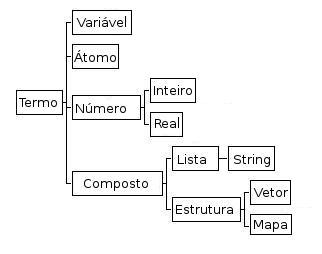
\includegraphics[width=.6\textwidth]{figures/tipos_dados_picat_traduzido.jpg}
\caption{Hierarquia dos tipos de dados $=$ termos}
\label{Hiera}
\end{figure}

\end{frame}

%%%%%%%%%%%%%%%%%%%%%%%%%%%%%%%%%%%%%%%%%%%%%%%%%%%%%%%%%%%%%%%%%%%%%
\subsection{Tipos Simples}
\begin{frame}
    \frametitle{Variável}
   
   \begin{itemize}
     \item Em PICAT começam por letras MAIÚSCULAS. Ex: Velocidade, TEMPO, etc
     \item Como na matemática, armazenam valores, outras variáveis, estruturas complexas, etc

     \item Diferente das outras LPs: não possuem endereço de memória fixo

     \item A variável está instanciada (\textit{bound}) ou está livre (\textit{free})
     \item Uma vez instanciada, permanece com um determinado valor na chamada corrente
     
   \end{itemize}
   
  
   
\end{frame}


\begin{frame} [allowframebreaks=0.9]

    \frametitle{Exemplo de Variável}
   
  \begin{itemize}
    \item \texttt{X = 34, println(xzinho = X).}
    \item \texttt{X = 34, Y = 34, Z := X + Y.}
    \item \texttt{X = 34, println(xzinho = X), X := 17, println(xzinho = X).}
    \item Mas \texttt{X = 34,  X = 17, println(xzinho = X).}\\ logo
    \texttt{X = 34} é diferente de \texttt{X := 34}
    \item Assim, cuidar em PICAT no caso de:
    
    \begin{itemize}
      \item \texttt{\textbf{=}} é o operador de unificação ou casamento de variáveis livres
      \item \texttt{\textbf{:=}} é a atribuição das LPs clássicas
      \item \texttt{\textbf{==}} é a comparação entre dois termos
      
    \end{itemize}
  
  \item Predicado útil: \texttt{bind\_vars(\{X,Y,Z\}, 56.789 )}\\
  X = 56.789000000000001\\
  Y = 56.789000000000001\\
  Z = 56.789000000000001\\
  yes

\item Igualmente: \texttt{X = 234.56, copy\_term(X) = Y}\\
  X = 234.560000000000002\\
  Y = 234.560000000000002\\
  yes\\
  
  \textcolor{red}{$\Rightarrow $ Caso X se encontre unificado (venha com um casamento de padrão), e se  deseje alguma modificação a partir de X. Então realiza-se uma cópia do   mesmo para uma variável temporária Y, e modifica-se Y.}

\item Pode-se utilizar também o \texttt{bind\_vars}:\\
X = 321.01, bind\_vars(\{Y\}, X), Y:= Y + 321.\\
X = 321.009999999999991\\
Y = 642.009999999999991\\
yes

\item Outros predicados úteis: \texttt{var}, \texttt{nonvar} (retorna \texttt{\textit{yes}} se a variável não estiver livre). Exemplo:\\
\texttt{( X = 7, nonvar(X) ) , var(Y) }\\
\texttt{X = 7}\\
yes -- nos dois casos eram \textit{true}\\

\item Uma variável atribuída tem um \textit{mapa} com um par de valores ligados a ela: o seu conteúdo(s) e estado (\textit{true/false}).

\item Ver manual alguns predicados específicos para este fim!

  \end{itemize}
    
\end{frame}
%%%%%%%%%%%%%%%%%%%%%%%%%%%%%%%%%%%%%%%%%%%%%%%%%%%%%%%%%%%%%%%%%%%%%

\begin{frame}
    \frametitle{Atribuição}


   
\begin{itemize}
  \item   \texttt{X := 7, X := X + 7, X := X + 7.}\\
     \texttt{X = 21}
     
   \item  \textcolor{red}{A atribuição tem um escopo local ao predicado em questão!}

   \item Enfim, cuidar do que se deseja modificar e retornar!
\end{itemize}

\end{frame}

%%%%%%%%%%%%%%%%%%%%%%%%%%%%%%%%%%%%%%%%%%%%%%%%%%%%%%%%%%%%%%%%%%%%%

\begin{frame}
    \frametitle{Átomo}
   
   \begin{itemize}
    
     \item Um átomo é uma constante simbólica
     \item Seu nome pode ser representado tanto com aspas simples ou sem
     \item Tamanho de um átomo $\le 1000$ caracteres
     \item Exemplos: \texttt{x\_20 , 'x\_21' , 'a' , a , abacate}, etc
     \item Mas \texttt{'ab'== ab} são iguais

   \end{itemize}
      
\end{frame}

%%%%%%%%%%%%%%%%%%%%%%%%%%%%%%%%%%%%%%%%%%%%%%%%%%%%%%%%%%%%%%%%%%%%%

\begin{frame}
    \frametitle{Exemplo de Átomos}
   
  \begin{itemize}
    
     \item \texttt{atom('x') , atom(x)} cuidar com 
     \textcolor{red}{\texttt{atom('x') == atom(x)}}
     \item \texttt{atom\_chars('x') = X} 
     \item \texttt{chr(68) = Valor}
     \item \texttt{ord('D') = Valor} -- inverso da anterior
     \item \texttt{digit(1)} $\equiv$ \textit{no} e \texttt{digit('1')} $\equiv$ \textit{yes}
     \item \texttt{length(udesc) = X}
     \item \texttt{len(udesc) = X}
     
  \end{itemize}
  
\end{frame}

%%%%%%%%%%%%%%%%%%%%%%%%%%%%%%%%%%%%%%%%%%%%%%%%%%%%%%%%%%%%%%%%%%%%%

\begin{frame}
    \frametitle{Números}
    
    \begin{itemize}
      \item Um número é um átomo inteiro ou real
      
      \item Um número inteiro pode ser representado na forma 
            decimal, binária, 
            octal ou hexadecimal
      
      \item Um úmero real usa o ponto no lugar da vírgula para separar 
      os valores depois de zero como: \texttt{3.1415}
      
      
    \end{itemize}
    
\end{frame}

%%%%%%%%%%%%%%%%%%%%%%%%%%%%%%%%%%%%%%%%%%%%%%%%%%%%%%%%%%%%%%%%%%%%%

\begin{frame}
    \frametitle{Exemplo de Números Reais e Inteiros}
   
  \begin{itemize}
    \item  \texttt{X = 3 , number(X).}
    \item  \texttt{X = 3 , Y = 4 , X < Y.}
    \item \texttt{number\_chars(45) = X}\\ 
    \pause
    \texttt{X = ['4','5']}

    \item \texttt{number\_codes(45) = X}\\
    \pause
    \texttt{X = [52,53]}
    
    \item \texttt{real(5.4321)}
    
    \item \texttt{int(321) $\equiv$ integer(321)} são predicados!
    
  \end{itemize}
  
   
\end{frame}


%%%%%%%%%%%%%%%%%%%%%%%%%%%%%%%%%%%%%%%%%%%%%%%%%%%%%%%%%%%%%%%%%%%%%

\subsection{Tipos Compostos}
\begin{frame} [allowframebreaks=0.9]
    \frametitle{Tipos Compostos}
        
    \begin{description}
      \item[Lista:] sequência de termos 
           %%% \lstinputlisting{../xxxxx.pi}    
           \begin{itemize}
          \item \texttt{ L = [ a, b, c] , length(L) = X}
          \item \texttt{ L = [ a, b, c] , L.length = X}
          \item \texttt{ L = [ a, b, c] , get(L,length) = X}
          \item Em breve uma aula sobre construir funções e predicados sobre listas 
          \item Há uma  quantidade de funções e predicados sobre listas embutidos (prontos para uso)
           \end{itemize}
           
             
      
       \item[Strings:] uma lista de carácteres\\
       \texttt{ X = "Oi bom dia!"}\\
       \texttt{ X = ['O',i,' ',b,o,m,' ',d,i,a,!]}
        
     
     \begin{itemize}
      \item \texttt{X = "Oi bom dia!", to\_uppercase(X) =  Y}
       \item Predicado: \texttt{string(X)}
      \end{itemize}        
      
       \item[Estrutura:] um modo de organizar dados heterogêneos em um único termo. 
       \begin{itemize}
         \item Uma estrutura tem o formato \texttt{\$est($t_1, t_2, ..., t_n$)},
       onde \texttt{est} é um átomo e $n$ é a aridade da estrutura.
         \item O \$ é usado para diferenciar uma estrutura de uma função em um dos argumentos
         do predicado (sim, uma função pode ser um argumento de um predicado)
         \item Cuidados nos \textcolor{red}{casamentos dos termos}. Veja o exemplo:
         \end{itemize}
   
    \end{description}
     
     Execute: \textcolor{blue}{struct\_ex01.pi}\\
     \lstinputlisting{../struct_ex01.pi}    
     
     \newpage
     
     
    \begin{description}      
%%[allowframebreaks=0.9]
     
      
       \item[Vetores:] 
           %%% \lstinputlisting{../struct_ex01.pi}    
           
           \begin{itemize}
  \item Um vetor ou \textit{array} tem o formato \texttt{\{$t_1,…,t_n$\}}, o qual é um caso especial de uma estrutura delimitada por  '\{  \}’ e aridade $n$
  \item Tem seu comprimento delimitado na memória e tempo de acesso 
  constante a seus elementos
  
  \item Análogo aos vetores de outras linguagens com uma notação e funções bem fáceis de usar. Exemplo \texttt{Vetor[7]} acessa a 7a. posição deste vetor unidimensional
             
  \item Para criar um array:\\
       \textbf{\textcolor{red}{\texttt{new\_array($D_1, …, D_n$) = Vetor}}} onde $D_1, …, D_n$ especificam as dimensões do mesmo. Atualmente, $n \le 10$ (matrizes de  10 dimensões $\Rightarrow $ mais do que suficiente!) 
             
    \item Como sua implementação tem origem das listas, é de se esperar que: $Listas \Leftrightarrow Vetores$           
    
 \item Logo, há muitas funções e predicados de listas  que facilitam o tratamento  com vetores
    
  \item Mas, \textcolor{red}{algumas estão prontas apenas para vetores unidimensionais}. Cuidado aqui. Veja o exemplo para superar estas dificuldades.  
            
% \item  A principal diferença é que listas crescem de modo inderterminado  e vetores não!    
           \end{itemize}
 \end{description}
           
%%%%%% CODE           

         Execute: \textcolor{blue}{array\_example01.pi}\\  
         \lstinputlisting{../array_example01.pi}  

   \begin{description}        
           
       \item[Mapas:] (em breve)
  
       \item[Conjuntos:] (em breve)
       
    \end{description}

\end{frame}

%%%%%%%%%%%%%%%%%%%%%%%%%%%%%%%%%%%%%%%%%%%%%%%%%%%%%%%%%%%%%%%%%%%%%


%%%%%%%%%%%%%%%%%%%%%%%%%%%%%%%%%%%%%%%%%%%%%%%%%%%%%%%%%%%%%%%%%%%%%
\begin{comment}

%%%%%%%%%%%%%%%%%%%%%%%%%%%%%%%%%%%%%%%%%%%%%%%%%%%%%%%%%%%%%%%%%%%%%

\begin{frame}
    \frametitle{Estruturas de Controle}
        
     \lstinputlisting{../estrutura_if_then_ex01.pi}
    
\end{frame}

%%%%%%%%%%%%%%%%%%%%%%%%%%%%%%%%%%%%%%%%%%%%%%%%%%%%%%%%%%%%%%%%%%%%%

\begin{frame}
    \frametitle{Entradas e Saídas}
  
  
  \lstinputlisting{../media_2_reais.pi}
  
\end{frame}
\end{comment}

%%%%%%%%%%%%%%%%%%%%%%%%%%%%%%%%%%%%%%%%%%%%%%%%%%%%%%%%%%%%%%%%%%%%%


%%%%%%%%%%%%%%%%%%%%%%%%%%%%%%%%%%%%%%%%%%%%%%%%%%%%%%%%%%%%%%%%%%%%%
%%%%%%%%%%%%%%%%%%%%%%%%%%%%%%%%%%%%%%%%%%%%%%%%%%%%%%%%%%%%%%%%%

\section{Conclusão}
\begin{frame}
    \frametitle{Conclusão}
    \begin{itemize}
    \item Os principais tipos de dados foram apresentados
    
    \item Apresentamos o uso de predicados e funções destes TDs, 
    e extensões. Exemplo: uso da função \texttt{sum-1D} para \texttt{sum-2D}
    
    \item Próximo vídeo: laços, predicados e funções

    %\item Uso muito bom quanto a: Planejamento, Programação por Restrição e PD (diretamente)
    
   % \item Todos problemas NPs-Completos!
    \end{itemize}
\end{frame}

%%%%%%%%%%%%%%%%%%%%%%%%%%%%%%%%%%%%%%%%%%%%%%%%%%%%%%%%%%%%%%%%%%%%%

%\section{Referências}
\begin{frame}
    \frametitle{Referências}
    \begin{itemize}
    \item O \textit{User Guide} que está no diretório  \texttt{doc/} da instalação em \LaTeX 
    \item Em \url{http://pic at-lang.org/} -- \textit{User Guide on-line} está lá também
    
     \item Meu GitHub $\Rightarrow $ \url{https://github.com/claudiosa/CCS/tree/master/picat}
    
    \item Assinem o fórum do PICAT(em inglês: respondo lá também)

    \item Sítio do Hakan  Kjellerstrand  $\Rightarrow $ \url{http://www.hakank.org/picat/}
    \item Sítio do Roman Barták  $\Rightarrow $ \url{http://ktiml.mff.cuni.cz/~bartak/}
    \item Sítio do Sergii Dimychenko  $\Rightarrow $ \url{http://sdymchenko.com/blog/2015/01/31/ai-planning-picat/}
    
    \end{itemize}
\end{frame}

%%%%%%%%%%%%%%%%%%%%%%%%%%%%%%%%%%%%%%%%%%%%%%%%%%%%%%%%%%%%%%%%%%%%%
\section{Agradecimentos}
\begin{frame}
 \frametitle{Agradecimentos}

\begin{itemize}
  \item Marlon Henry Schweigert
  \item Paulo Victor Aguiar
  \item Rogério Eduardo da Silva
  
\end{itemize}

\end{frame}

%%%%%%%%%%%%%%%%%%%%%%%%%%%%%%%%%%%%%%%%%%%%%%%%%%%%%%%%%%%%%%%%%%%%%
%\section{Questionário}
\begin{frame}
    \frametitle{Obrigado}

\begin{figure}[!ht]
\centering

\includegraphics[height=0.45\textheight]{figures/meu_logo_picat.pdf}
%%\caption{Hierarquia dos Tipos de dados} [width=.7\textwidth]
%%\label{Hiera}
\end{figure}
 Retornem os comentários para o próximo vídeo!!!


\end{frame}

\end{document}
